\documentclass[letterpaper,12pt]{article}
\usepackage{mathtools}
\DeclarePairedDelimiter\abs{\lvert}{\rvert}     %serve per mettere il modulo 
\usepackage{booktabs}
\usepackage{bm}
\usepackage{textcomp}
\usepackage{colortbl}
\usepackage{tabularx}
\usepackage{textcomp}
\usepackage{siunitx}
\usepackage{booktabs}
\usepackage{enumitem}
\usepackage{xcolor}
\usepackage{fancyhdr}
\usepackage{caption}
\usepackage{changepage}
\usepackage{amsmath} 
\usepackage{subcaption}
\usepackage{graphicx}
\usepackage[table]{xcolor} 
\usepackage{colortbl}
\usepackage[margin=1in,letterpaper]{geometry} % decreases margins
\usepackage{cite} % takes care of citations
\usepackage[hidelinks]{hyperref} % adds hyper links inside the generated pdf file
\usepackage{siunitx} % provides the \SI{}{} command for proper typesetting of units
% Define the colors
\definecolor{linkcolor}{RGB}{0, 102, 204}
\definecolor{citecolor}{RGB}{34, 139, 34}
\definecolor{urlcolor}{RGB}{255, 69, 0}
\definecolor{wavelength_406}{RGB}{129, 0, 204}
\definecolor{wavelength_447}{RGB}{0, 53, 255} 
\definecolor{wavelength_402}{RGB}{131, 0, 188}  
\definecolor{wavelength_501}{RGB}{0, 255, 135}
\definecolor{wavelength_440}{RGB}{0, 0, 255}   
\definecolor{wavelength_513}{RGB}{21, 255, 0}   
\definecolor{wavelength_nan}{RGB}{210,210,210} 
\definecolor{wavelength_540}{RGB}{129, 255, 0}  
\definecolor{wavelength_458}{RGB}{0, 113, 255}  
\definecolor{wavelength_568}{RGB}{219, 255, 0}
\definecolor{wavelength_587}{RGB}{255, 233, 0} 
\definecolor{wavelength_585}{RGB}{255, 239, 0} 
\definecolor{wavelength_472}{RGB}{0, 178, 255}
\definecolor{wavelength_667}{RGB}{235, 0, 0}  
\definecolor{wavelength_676}{RGB}{227, 0, 0}  
\definecolor{wavelength_640}{RGB}{255, 33, 0}  
\definecolor{wavelength_696}{RGB}{209, 0, 0}
\definecolor{wavelength_449}{RGB}{0, 65, 255}
\definecolor{wavelength_503}{RGB}{0, 255, 110}
\definecolor{wavelength_581}{RGB}{255, 252, 0}


% Setup hyperref
\hypersetup{
    colorlinks=false, % colored links
    linkcolor=linkcolor, % color for internal links
    citecolor=citecolor, % color for citations
    urlcolor=urlcolor, % color for URLs
}
\fancypagestyle{logoheader}{
    \fancyhf{}
    \fancyhead[L]{
\includegraphics[width = 3cm]{infn-art-science-universita-degli-studi-di-milano-bicocca-maintainer-universita-studi-milano-bicocca.png}}
    \renewcommand{\headrulewidth}{0pt}
    }
\usepackage{blindtext}
\graphicspath{{immagini/}}
%Required for inserting images
%++++++++++++++++++++++++++++++++++++++++
%Margini 


\begin{document}


\title{{\small Università degli studi Milano-Bicocca  Dipartimento di Fisica - Laboratorio II }\\
	Esperienza Ottica - Interferometro}
\author{F. Ballo, S. Franceschina, S. Dolci - Gruppo T1 39}
\date{\today}
\maketitle
\thispagestyle{logoheader}


\begin{abstract}
	Nella seguente relazione vengono presentati i risultati ottenuti dalla sesta esperienza del corso di 
    Laboratorio II riguardante l'analisi di fenomeni ottici.
    L'obiettivo di questa esperienza è quello di riprodurre due esperimenti di interferometria: Fabri-Perot e Michelson.
    Per ciascuno di questi setup riprodotti in laboratorio lo scopo è quello di verificare certe relazioni, che occorrono
    nel momento in cui raggi luminosi interferiscono tra loro, dalle quali è possibile ricavare informazioni utili come 
    la lunghezza d'onda della sorgente.
	\begin{adjustwidth}{-1cm}{-1cm}
	\end{adjustwidth}
\end{abstract}
\tableofcontents
\newpage

\section{Configurazione setup esperienza}
Per le misure di questa esperienza abbiamo utilizzato:

\begin{itemize}
    \item Un interferometro di precisione PASCO scientific Modello OS-9255A/OS-9258A , \href{https://www.pasco.com/products/lab-apparatus/light-and-optics/advanced-optics/os-9255}{[link]}
    \item Sorgente: laser monocromatico He-Ne con lunghezza d'onda $\lambda = \SI{632.8}{\nano\meter}$.
    \item Lente divergente: lente da 18mm.
    \item Specchi compresi nella dotazione PASCO
\end{itemize}


\section{Fabry-Perot}
La prima parte dell'esperienza consiste nella verifica della legge che descrive
i massimi di interferenza, visibili quando due sorgenti si sommano in fase. 
Per farlo abbiamo montanto l'interferometro in configurazione Fabry-Perot:

\begin{figure}[ht]
    \centering
    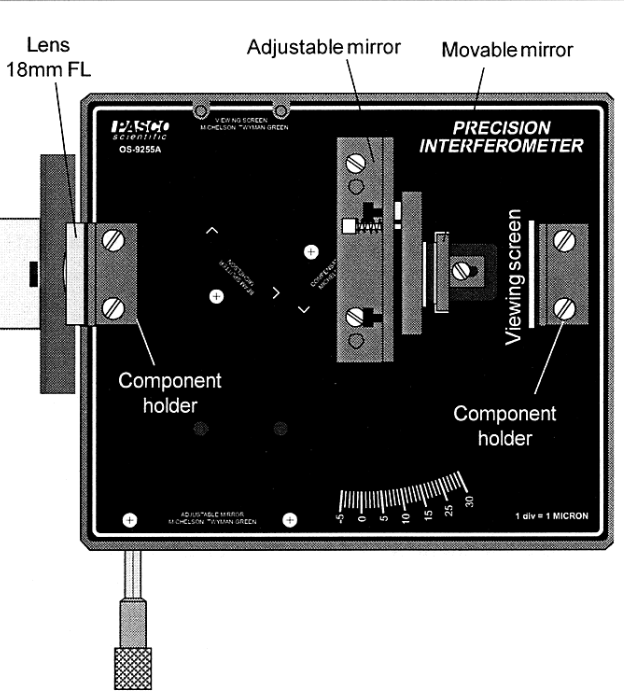
\includegraphics[width=0.4\textwidth]{InterferometroFabry.png}
    \caption{Configurazione Fabry-Perot.}
    \label{fig:fabry-perot config}
\end{figure}

L luce del fascio laser incide contro una lente divergente e entra nella cavità di Fabry-Perot, ovvero due specchi semiriflettenti 
distanziati $d$. Le riflessioni successive tra i due specchi formano la figura di interferenza sullo schermo, posto
a circa un metro di distanza. \\ 
È interessante notare come, per ricavare le relazioni che verranno utilizzate per descrivere il fenomeno, si 
introduca l'ipotesi che i raggi luminosi siano paralleli tra di loro nell'ingresso della cavità, nonostante la 
presenza di una lente divergente. Abbiamo motivato questa ipotesi osservando che la lente divergente è posta
molto vicina alla cavità, e quindi la divergenza dei raggi luminosi è trascurabile. Non si può dire lo stesso per 
quanto riguarda i raggi che incidono sullo schermo, essi infatti sono considerati divergenti perchè la distanza tra
schermo e specchio è significativa.\\
Un'altra osservazione importante riguarda gli angoli delle frange di interferenza. 
Per l'angolo $\theta$, quello riportato in figura \ref{fig:fabry_perot_scheda},
\begin{figure}[h!]
    \centering
    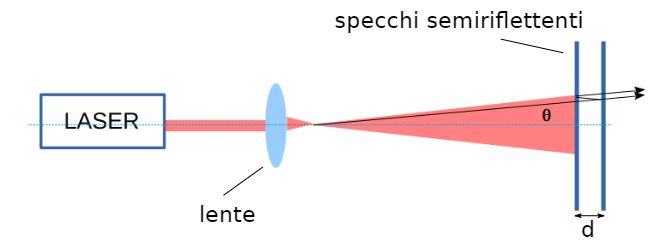
\includegraphics[width=0.4\textwidth]{fabry_perot_config.JPG}
    \caption{Configurazione Fabry-Perot.}
    \label{fig:fabry_perot_scheda}
\end{figure}

abbiamo posto il vertice nel fuoco della lente divergente (18mm avanti) e misurato la distanza tra tale fuoco e lo schermo. 
In questo modo, misurando in seguito la distanza tra il centro della figura di interferenza e la frangia, 
è possibile calcolare l'angolo $\theta$ come l'arcotangente del rapporto tra le due distanze. In ogni caso, tali 
considerazioni sono state rilevanti solo per questa prima parte dell'esperienza, in cui era richiesto di verificare 
la legge \ref{eq:fabry_perot} confrontando i valori di angoli attesi con quelli misurati. Per tutte le altre esperienze 
abbiamo potuto considerare $\theta \approx 0$ e quindi $\cos(\theta) \approx 1$ poichè lo schermo si trova 
a una grande distanza dalla sorgente puntiforme.

\subsection{Verifica della legge di interferenza}

In questa prima parte dell'esperienza abbiamo cercato di verificare
la seguente legge di interferenza, che descrive quando i due raggi luminosi interferiscono in fase:

\begin{equation}
    \delta_r \frac{\lambda}{2 \pi} + 2d \cos(\theta) = N \lambda
    \label{eq:fabry_perot}
\end{equation}

$d$ è la distanza tra i due specchi, $\delta_r$ rappresenta lo sfasamento , $\theta$ è l'angolo di incidenza della luce, $N$ è l'ordine di interferenza e $\lambda$ 
è la lunghezza d'onda del laser sorgente. \\
Per verificarla abbiamo deciso di invertire la relazione in modo da evidenzare la dipendenza di $\cos(\theta)$ dalle
altre variabili, ricavando la relazione \ref{eq:fabry_perot_cos}:

\begin{equation}
    \cos(\theta) = \frac{N \lambda}{2d} - \frac{\delta_r \lambda}{4 d \pi}
    \label{eq:fabry_perot_cos}
\end{equation}
Dopo aver verificato le opportune calibrazioni del laser, delle lenti e dello specchio,
abbiamo misurato il diametro dei cerchi di interferenza con un calibro e calcolato così il coseno dell'angolo $\theta$.\\

\subsection{Analisi Dati legge di interferenza}
Di seguito riportiamo i dati raccolti in laboratorio; la distanza dello schermo dalla sorgente è pari a $D = 1.37 \pm0.01 m$, assumendo come punto sorgente il fuoco della lente 
(18mm). Successivamente per la verifica del modello abbiamo eseguito un'interpolazione con la legge \ref{eq:fabry_perot_cos}, mantenendo come 
parametri liberi $\delta_r$ e $d$.\\
Abbiamo ripetuto tale misura per quattro volte, variando d, al fine di poter verificare in più configurazioni la 
legge \ref{eq:fabry_perot}.\\
Riportiamo di seguito i grafici dei fit ottenuti per ciascuna delle misurazioni in figura \ref{fig:verifica_fabry_perot}:

%Da discutere gli errori (anche in relazione ai valori di chi quadro ottenuti)

\begin{figure}[h!]
    \centering
    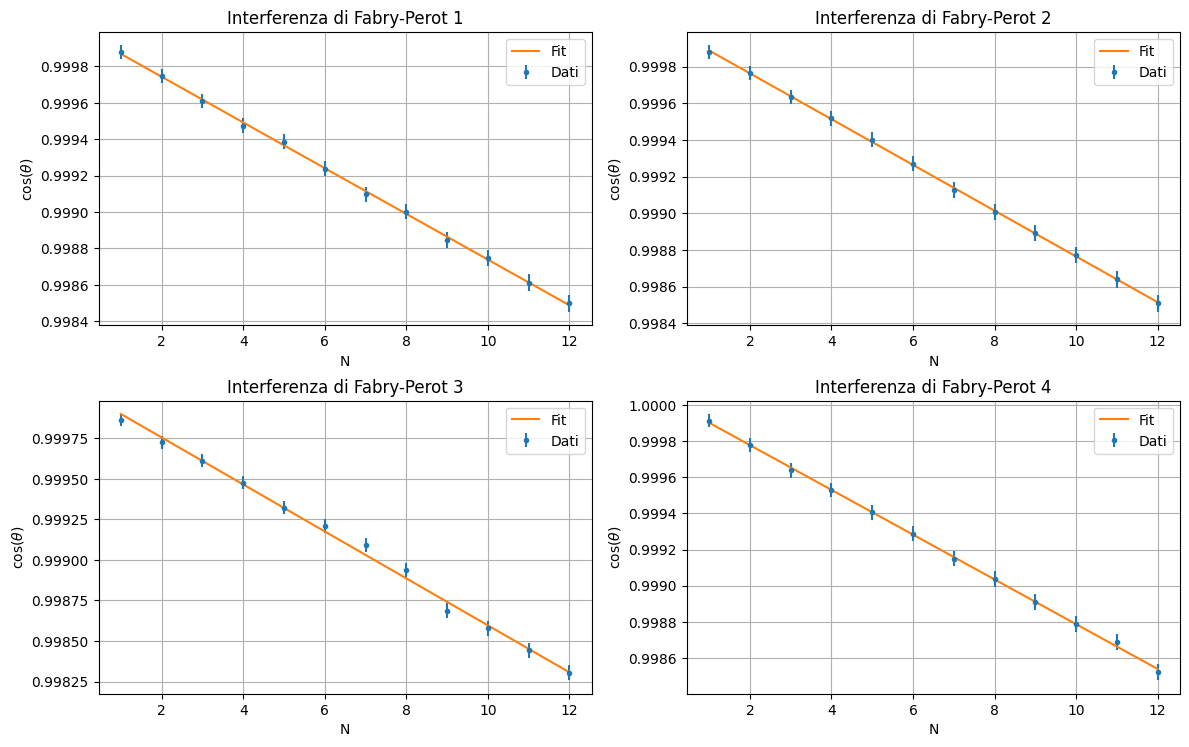
\includegraphics[width=1\textwidth]{verifica_fabry_perot.png}
    \caption{Interpolazioni della legge \ref{eq:fabry_perot_cos}.}
    \label{fig:verifica_fabry_perot}
\end{figure}

Nella tabella \ref{tab:dati_interpolazioni_FP} riportiamo i valori ottenuti per i parametri $\delta_r$ e $d$ 
con i relativi errori, insiema ai valori del $\tilde{\chi}^2$ e p-value trovati dalle interpolazioni.

%Da discutere le unità di misura dei parametri.

\begin{table}[h!]
    \centering
    \begin{tabular}{|c|c|c||c|c|c|}
    \hline
    \multicolumn{3}{|c||}{\textbf{Interpolazione 1}} & \multicolumn{3}{c|}{\textbf{Interpolazione 2}} \\
    \hline
    \textbf{Parametro} & \textbf{Valore} & \textbf{Errore} & \textbf{Parametro} & \textbf{Valore} & \textbf{Errore} \\
    \hline
    \text{d} & 0.00252 & 4.82e-07 & \text{d} & 0.00254 & 4.83e-07 \\
    \textbf{$\delta_r$} & 5.01e+04 & 9.56 & \textbf{$\delta_r$} & 5.04e+04 & 9.58 \\
    \textbf{$\tilde{\chi}^2$} & 0.00307 & \textbf{p-value :} 1 & \textbf{$\tilde{\chi}^2$} & 0.0398 & \textbf{p-value :} 1 \\
    \hline
    \multicolumn{3}{|c||}{\textbf{Interpolazione 3}} & \multicolumn{3}{c|}{\textbf{Interpolazione 4}} \\
    \hline
    \textbf{Parametro} & \textbf{Valore} & \textbf{Errore} & \textbf{Parametro} & \textbf{Valore} & \textbf{Errore} \\
    \hline
    \text{d} & 0.00219 & 4.22e-07 & \text{d} & 0.00255 & 4.84e-07 \\
    \textbf{$\delta_r$} & 4.34e+04 & 8.36 & \textbf{$\delta_r$} & 5.06e+04 & 9.60 \\
    \textbf{$\tilde{\chi}^2$} & 0.75 & \textbf{p-value :} 0.678 & \textbf{$\tilde{\chi}^2$} & 0.0756 & \textbf{p-value :} 1 \\
    \hline
    \end{tabular}
    \caption{Dati, deviazioni e test $\tilde{\chi}^2$ con p-value, suddivisi per interpolazione.}
    \label{tab:dati_interpolazioni_FP}
    \end{table}

\subsection{Calibrazione micrometro - Frange}
L'interferometro in configurazione Fabry-Perot è dotato di un micrometro che permette 
di variare la distanza tra i due specchi $\Delta d$.
Quando questa $\Delta d$ varia, varia anche il cammino ottico dei raggi luminosi e quindi la posizione delle frange di interferenza.
La legge che lega questo spostamento è la seguente:
    \begin{equation}
        \Delta d = \frac{\Delta N \cdot \lambda}{2 \cdot \cos(\theta)}
        \label{eq:micrometro}
    \end{equation}

Misurando quante frange scorrono sullo schermo è possibile risalire a una misura di alta precisione
del $\Delta d$ e quindi calibrare il micrometro.\\
Dopo aver registrato una posizione di partenza inziale dello specchio abbiamo scelto $\Delta d_\text{nomio} = 20\text{\SIUnitSymbolMicro m}$ come passo del nomio,
 il coseno dell'angolo $\theta$ approssimato a circa 1, dato che assumiamo incidenza normale.
Infine abbiamo ripetuto la misura più volte, sempre ripartendo
dalle stessa posizione iniziale cercando così di ridurre l'errore 
statistico e ottenendo una media per la distanza.


%Riguardiamo gli errori
\subsection{Analisi Dati calibrazione micrometro}
Riportiamo in seguito i dati ottenuti dalle misurazioni:
\begin{table}[h!]
    \centering
    \begin{tabular}{|c|c|c|c|c|}
    \hline
    \textbf{Misura} & \textbf{Frange $\Delta N$} & \textbf{Distanza $\Delta d$} & \textbf{Errore $\pm\sigma$}  \\
    \hline
    1 & 61 & 19,300 & 0.003 \\
    2 & 64 & 20,249 & 0.003 \\
    3 & 59 & 18,667 & 0.003 \\
    4 & 60 & 18,984 & 0.003 \\
    5 & 60 & 18,984 & 0.003 \\
    5 & 64 & 20,249 & 0.003 \\
    \hline
    \end{tabular}
    \caption{Dati raccolti per la calibrazione del micrometro.}
    \label{tab:calibrazione_micrometro}
    \end{table}

Riportiamo in seguito per la stima della distanza il valor medio e la deviazione standard $\Delta d_\text{mis} = 19.41 \pm0.07\text{\SIUnitSymbolMicro m} $
Le incertezze riportate nella tabella sono stati calcolate con l'oportuna formula di propagazione degli errori, riportiamo  inoltre
che per questi calcoli abbiamo utilizzato come valore tabulato la lunghezza d'onda del laser He-Ne $\lambda = \SI{632.8}{\nano\meter} \pm0.1$ \href{https://www.pasco.com/products/lab-apparatus/light-and-optics/advanced-optics/os-9255}{[link]}.
Abbiamo inoltre verificato che anche utilizzando $\lambda_\text{aria} = \frac{\lambda_0}{n_\text{aria}}$ dove $n_\text{aria} = 1,0003$ è l'indice di rifrazione dell'aria, la precisione della misura non cambia.

\subsection{Conclusioni Fabry-Perot}

\newpage
\section{Interferometro Michelson}
Nella seconda parte dell'esperienza abbiamo montato l'interferometro in configurazione Michelson, prima per verificare 
la calibrazione del micrometro (e confrontarla con Fabry-Perot), poi per effettuare altre misure sull'indice di rifrazione
dell'aria e del vetro.
\begin{figure}[h]
    \centering
    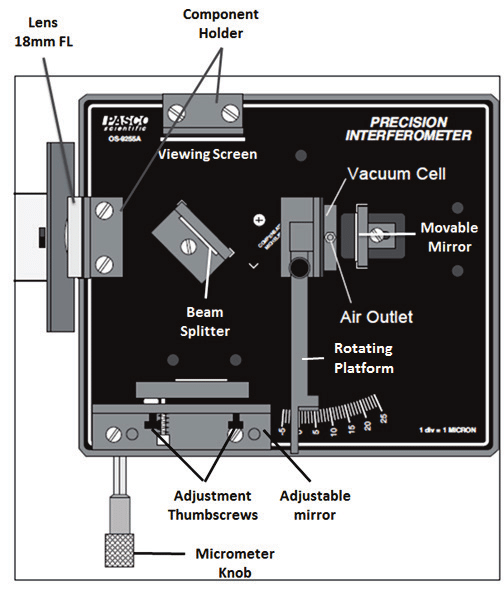
\includegraphics[width=0.4\textwidth]{Michelson_aria.png}
    \caption{Configurazione Michelson.}
    \label{fig:michelson config}
\end{figure}

\subsection{Verifica calibrazione micrometro}
Per eseguire la calibrazione del micrometro abbiamo seguito lo stesso procedimento utilizzato per Fabry-Perot, 
utilizzando la formula \ref{eq:micrometro} per calcolare la distanza $\Delta d$ tra i due specchi. Abbiamo ripetuto
la misura per quattro volte, spostando di $20 \text{\SIUnitSymbolMicro m}$ la distanza tra gli specchi, almeno in base a quanto segnato 
dal nonio. Riportiamo in tabella \ref{tab:calibrazione_micrometro_michelson} i risultati ottenuti. Come valore ottenuto
abbiamo deciso di considerare la media delle misure effettuate, ed errore la loro deviazione standard, in quanto 
misure non dotate di errore, perchè ricavate a partire da N e $\lambda$; ecco il valore di $\Delta d$ ottenuto: 
$\Delta d_\text{mis} = 1.94 \pm0.05\text{\SIUnitSymbolMicro m} $

\subsection{Misura indice rifrazione aria}
%aggiungere spiegazioni

Per risalire all'indice di rifrazione dell'aria, abbiamo utilizzato la formula \ref{eq:indice_rifrazione_aria}:
\begin{equation}
    n = 1 + \frac{\Delta N \lambda P_f}{2 d (P_i - P_f)}
    \label{eq:indice_rifrazione_aria}
\end{equation}

laddove $P_i$ e $P_f$ sono le pressioni iniziale e finale ($P_i = \SI{101.325}{\kilo\pascal}$), $\Delta N$ 
è il numero di frange contate, $d = \SI{0.03 \pm 0}{m}$ è la larghezza della camera a vuoto e $\lambda$ è la 
lunghezza d'onda del laser. Abbiamo ripetuto la misura per quattro volte, variando la pressione finale, e contando le 
frange di interferenza. Riportiamo in tabella \ref{tab:indice_rifrazione_aria_dati} i dati raccolti e in tabella 
\ref{tab:indice_rifrazione_aria} i valori ottenuti per l'indice di rifrazione dell'aria. Qui di seguito riportiamo
il valore ottenuto per l'indice di rifrazione dell'aria, con relativo errore $n_{aria} = 1.00035 \pm 0.00002$.\\
Gli errori sui singoli valori dell'indice di rifrazione sono stati calcolati con la formula di propagazione degli errori,
a, partire dalla relazione \ref{eq:indice_rifrazione_aria}, in cui $P_f$ ha come errore la sensibilità del manometro 
($\SI{2}{\kilo\pascal}$). L'errore sul valore medio è stato calcolato pesando gli errori delle singole misure, con la 
formula \ref{eq:errore_valore_medio}:
\begin{equation}
    \sigma_{\bar{x}} = \frac{1}{N} \sqrt{\sum_{i=1}^{N} (\sigma_i)^2}
    \label{eq:errore_valore_medio}
\end{equation}

Operando un test di compatibilità con il valore atteso (pari a $n_{aria} = 1.000292$), otteniamo una distanza in 
deviazioni standard pari a 2.37.\\

\subsection{Misura indice rifrazione vetro}



\subsection{Misura lunghezza d'onda con righello reticolo}





\section{Considerazioni sugli errori}
\label{sec:errori}

\subsection{Commenti finali}



\newpage
\section{Tabelle}

%Tabella per Michelson - Calibrazione micrometro

\begin{table}[h!]
    \centering
    \begin{tabular}{|c|c|}
    \hline
    \textbf{d} & \textbf{Valore} [$\mu m$] \\
    \hline
    $d_1$ & 1.96168e-05 \\
    $d_2$ & 1.8984e-05 \\
    $d_3$ & 1.8984e-05 \\
    $d_4$ & 1.8984e-05 \\
    $d_5$ & 2.02496e-05 \\
    \hline
    \end{tabular}
    \caption{Distanze tra gli specchi ottenute dalla formula \ref{eq:micrometro}.}
    \label{tab:calibrazione_micrometro_michelson}
\end{table}

%Tabella per Michelson - Indice di rifrazione aria
%valori acquisiti
\begin{table}[h!]
    \centering
    \begin{tabular}{|c|c|c|}
    \hline
    \textbf{$P_f$} & \textbf{Sensibilità} & \textbf{$\Delta N$} \\
    \hline
    76 & 2 & 16 \\
    80 & 2 & 18 \\
    50 & 2 & 11 \\
    42 & 2 & 9 \\
    \hline
    \end{tabular}
    \caption{Dati acquisiti per la misura dell'indice di rifrazione dell'aria.}
    \label{tab:indice_rifrazione_aria_dati}
\end{table}

%valori di n calcolati
\begin{table}[h!]
    \centering
    \begin{tabular}{|c|c|c|}
    \hline
    \textbf{Indice} & \textbf{$n_{aria}$} & \textbf{Errore} \\
    \hline
    1 & \num{1.00051} & \num{0.00005} \\
    2 & \num{1.00071} & \num{0.00008} \\
    3 & \num{1.00011} & \num{0.00008} \\
    4 & \num{1.00007} & \num{0.00005} \\
    \hline
    \end{tabular}
    \caption{Indici di rifrazione ottenuti dalla formula \ref{eq:indice_rifrazione_aria}.}
    \label{tab:indice_rifrazione_aria}
\end{table}


\end{document}